\chapter{Specifikacija programske potpore}
    \graphicspath{./dijagrami/}
		
	\section{Funkcionalni zahtjevi}
			
			\textbf{\textit{dio 1. revizije}}\\
			
			\textit{Navesti \textbf{dionike} koji imaju \textbf{interes u ovom sustavu} ili  \textbf{su nositelji odgovornosti}. To su prije svega korisnici, ali i administratori sustava, naručitelji, razvojni tim.}\\
				
			\textit{Navesti \textbf{aktore} koji izravno \textbf{koriste} ili \textbf{komuniciraju sa sustavom}. Oni mogu imati inicijatorsku ulogu, tj. započinju određene procese u sustavu ili samo sudioničku ulogu, tj. obavljaju određeni posao. Za svakog aktora navesti funkcionalne zahtjeve koji se na njega odnose.}\\
			
			
			\noindent \textbf{Dionici:}
			
			\begin{packed_enum}
				
				\item Dionik 1
				\item Dionik 2				
				\item ...
				
			\end{packed_enum}
			
			\noindent \textbf{Aktori i njihovi funkcionalni zahtjevi:}
			
			
			\begin{packed_enum}
				\item  \underbar{Aktor 1 (inicijator) može:}
				
				\begin{packed_enum}
					
					\item funkcionalnost 1
					\item funkcionalnost 2
					\begin{packed_enum}
						
						\item  podfunkcionalnost 1 
						\item  podfunkcionalnost 2
				
					\end{packed_enum}
					\item  funkcionalnost 3
					
				\end{packed_enum}
			
				\item  \underbar{Aktor 2 (sudionik) može:}
				
				\begin{packed_enum}
					
					\item funkcionalnost 1
					\item funkcionalnost 2
					
				\end{packed_enum}
			\end{packed_enum}
			
			\eject 
			
			
				
			\subsection{Obrasci uporabe}
				
				\textbf{\textit{dio 1. revizije}}
				
				\subsubsection{Opis obrazaca uporabe}
					\textit{Funkcionalne zahtjeve razraditi u obliku obrazaca uporabe. Svaki obrazac je potrebno razraditi prema donjem predlošku. Ukoliko u nekom koraku može doći do odstupanja, potrebno je to odstupanje opisati i po mogućnosti ponuditi rješenje kojim bi se tijek obrasca vratio na osnovni tijek.}\\
					

					\noindent \underbar{\textbf{UC$<$broj obrasca$>$ -$<$ime obrasca$>$}}
					\begin{packed_item}
	
						\item \textbf{Glavni sudionik: }$<$sudionik$>$
						\item  \textbf{Cilj:} $<$cilj$>$
						\item  \textbf{Sudionici:} $<$sudionici$>$
						\item  \textbf{Preduvjet:} $<$preduvjet$>$
						\item  \textbf{Opis osnovnog tijeka:}
						
						\item[] \begin{packed_enum}
	
							\item $<$opis korak jedan$>$
							\item $<$opis korak dva$>$
							\item $<$opis korak tri$>$
							\item $<$opis korak četiri$>$
							\item $<$opis korak pet$>$
						\end{packed_enum}
						
						\item  \textbf{Opis mogućih odstupanja:}
						
						\item[] \begin{packed_item}
	
							\item[2.a] $<$opis mogućeg scenarija odstupanja u koraku 2$>$
							\item[] \begin{packed_enum}
								
								\item $<$opis rješenja mogućeg scenarija korak 1$>$
								\item $<$opis rješenja mogućeg scenarija korak 2$>$
								
							\end{packed_enum}
							\item[2.b] $<$opis mogućeg scenarija odstupanja u koraku 2$>$
							\item[3.a] $<$opis mogućeg scenarija odstupanja  u koraku 3$>$
							
						\end{packed_item}
					\end{packed_item}
				
					
				\subsubsection{Dijagrami obrazaca uporabe}
					
					\textit{Prikazati odnos aktora i obrazaca uporabe odgovarajućim UML dijagramom. Nije nužno nacrtati sve na jednom dijagramu. Modelirati po razinama apstrakcije i skupovima srodnih funkcionalnosti.}
					
					
					\begin{figure}[h!]      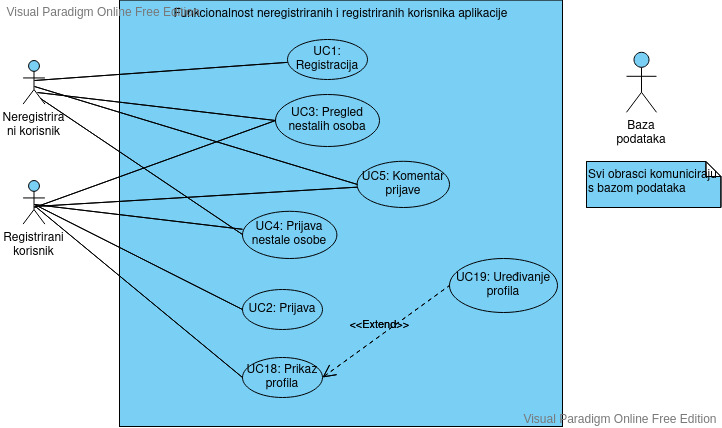
\includegraphics[width=\linewidth]{dijagrami/UML1.vpd.jpg}
					\caption{Dijagram obrasca uporabe, funkcionalnost neregistriranih i registriranih korisnika aplikacije}
	                \end{figure}
	                
				    \begin{figure}[H] 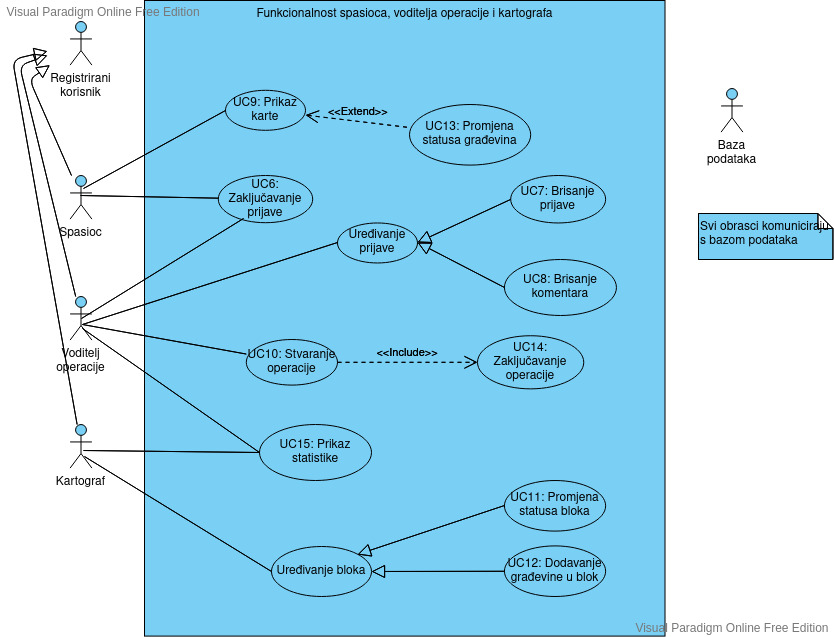
\includegraphics[width=\linewidth]{dijagrami/UML2.vpd.jpg}
				    \caption{Dijagram obrasca uporabe, funkcionalnost spasioca, voditelja operacije i kartografa}
				    \end{figure}
				    
				    \begin{figure}[H] 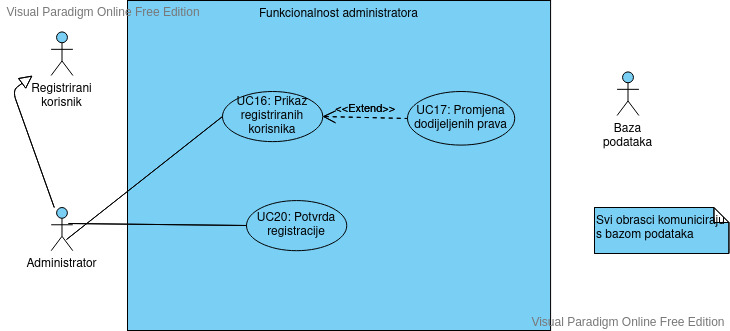
\includegraphics[width=\linewidth]{dijagrami/UML3.vpd.jpg} 
				    \caption{Dijagram obrasca uporabe, funkcionalnost administratora}
				    \end{figure} 
					
				\eject		
				
			\subsection{Sekvencijski dijagrami}
				
				\textbf{\textit{dio 1. revizije}}\\
				
				\textit{Nacrtati sekvencijske dijagrame koji modeliraju najvažnije dijelove sustava (max. 4 dijagrama). Ukoliko postoji nedoumica oko odabira, razjasniti s asistentom. Uz svaki dijagram napisati detaljni opis dijagrama.}
				\eject
	
		\section{Ostali zahtjevi}
		
			\textbf{\textit{dio 1. revizije}}\\
		 
			 \textit{Nefunkcionalni zahtjevi i zahtjevi domene primjene dopunjuju funkcionalne zahtjeve. Oni opisuju \textbf{kako se sustav treba ponašati} i koja \textbf{ograničenja} treba poštivati (performanse, korisničko iskustvo, pouzdanost, standardi kvalitete, sigurnost...). Primjeri takvih zahtjeva u Vašem projektu mogu biti: podržani jezici korisničkog sučelja, vrijeme odziva, najveći mogući podržani broj korisnika, podržane web/mobilne platforme, razina zaštite (protokoli komunikacije, kriptiranje...)... Svaki takav zahtjev potrebno je navesti u jednoj ili dvije rečenice.}
			 
			 
			 
	
